\chapter{Results}
\label{sec:results}

This chapter will present results to the reader.


\section{Evaluation of algorithm speed}
Table 4.1 shows the end-to-end time for the lane detection system currently implemented on the Raspberry Pi. Since the lane detection system need to be run in real time the speed of the algorithm is of great importance. This measurement includes the time for the image processing steps as well as the control structure and steering signal that goes to the servo motor that controls the steering. The mean fps is calculated as 1/mean time.


\begin{table}[H]
\centering
\caption{System End-to-end time}
\label{End-to-end time}
\begin{tabular}{@{} l *4c @{}}
\toprule
Image Resolution   & & & 384x288 & 640x480  \\ 
\midrule
 Mean time & & & 0.0422 & 0.0786 \\ 
 Mean fps & & & 23.714 & 12.724 \\
\bottomrule
 \end{tabular}
\end{table}


\ref{fig:The modified RC-car}

\begin{figure}[H]
  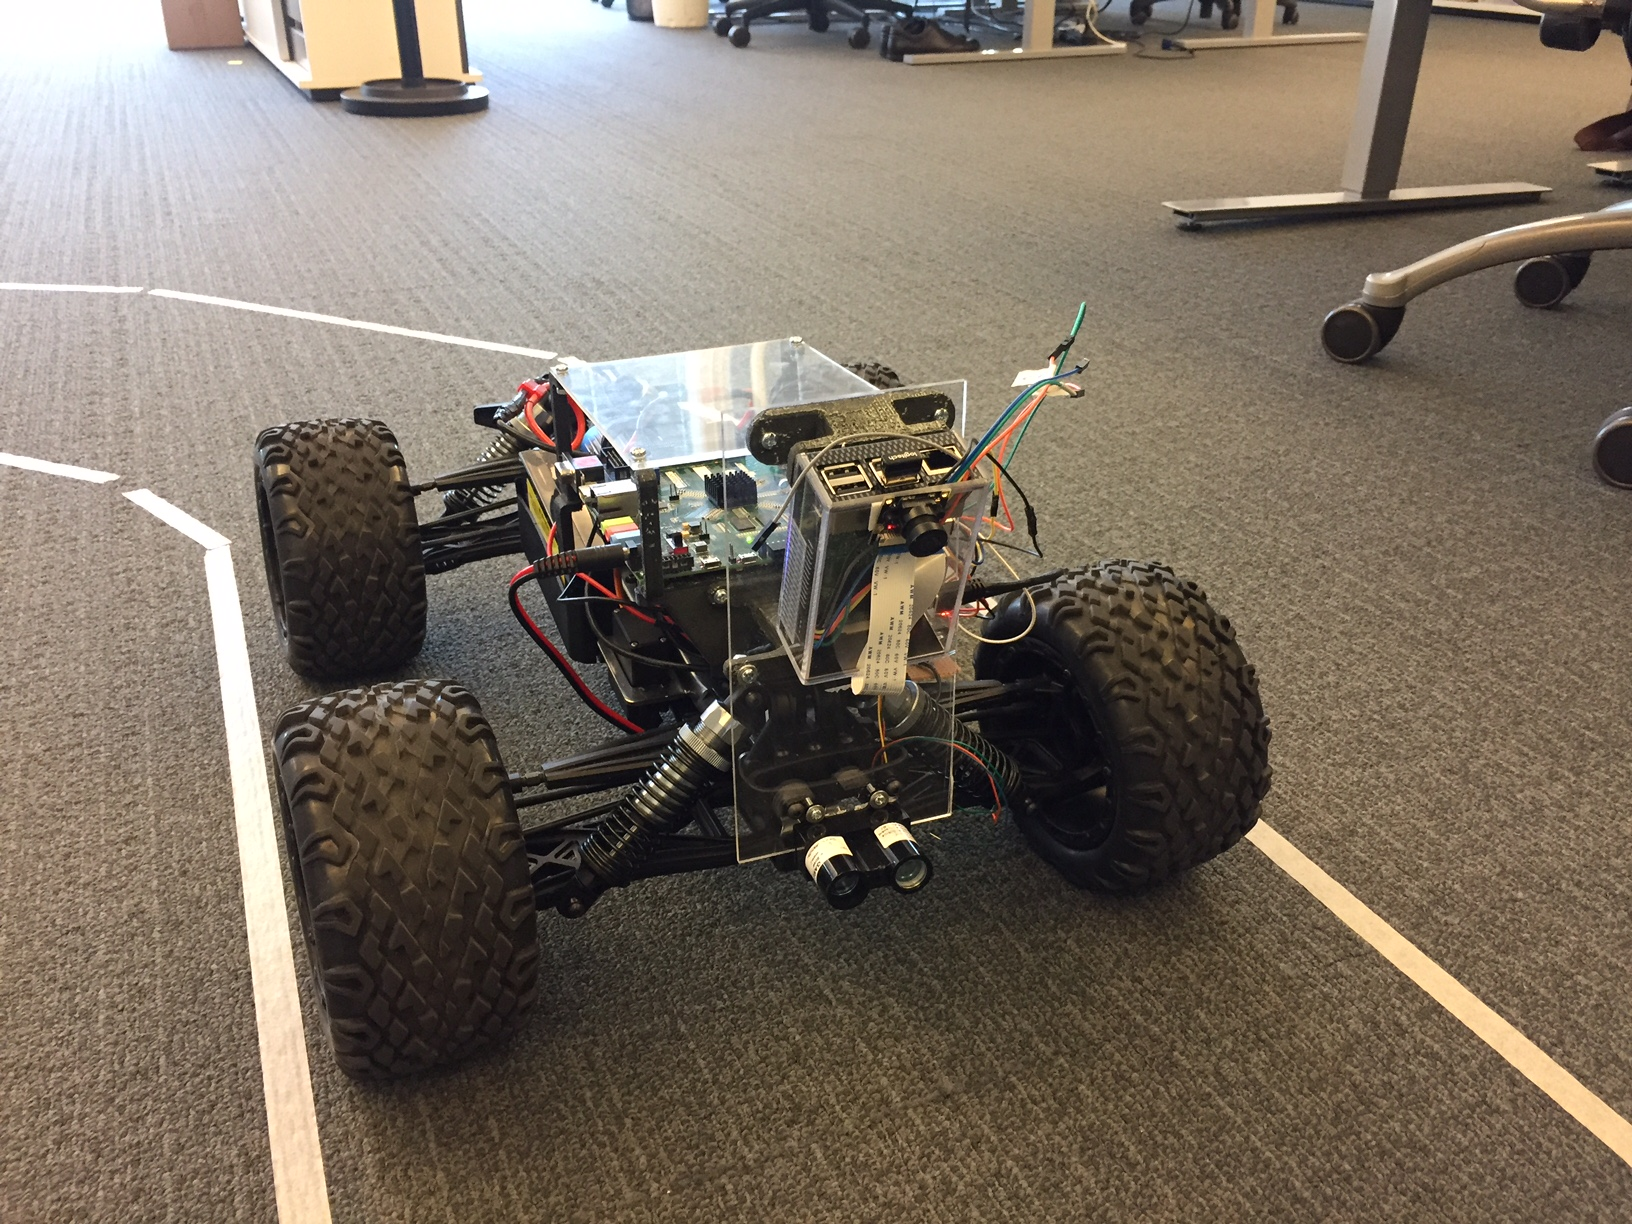
\includegraphics[width=\textwidth]{./img/utor.JPG}
  \centering
  \caption{The modified RC-car}
  \label{fig:The modified RC-car}
\end{figure}